
\section{Grundlagen}
Das ist der Grundlagenteil

% Hier beginnt ein neuer Absatz.
%Dies ist der zweite Absatz.
%
% Dann noch ein Unterabschnitt
%\subsection{Ein Unterabschnitt}
%Neuer Text in einem Unterabschnitt.
%
% Und noch ein ganz neuer Abschnitt
%\section{Der nächste Abschnitt}
%Noch mehr Text.

\begin{figure}[ht]
	\centering
	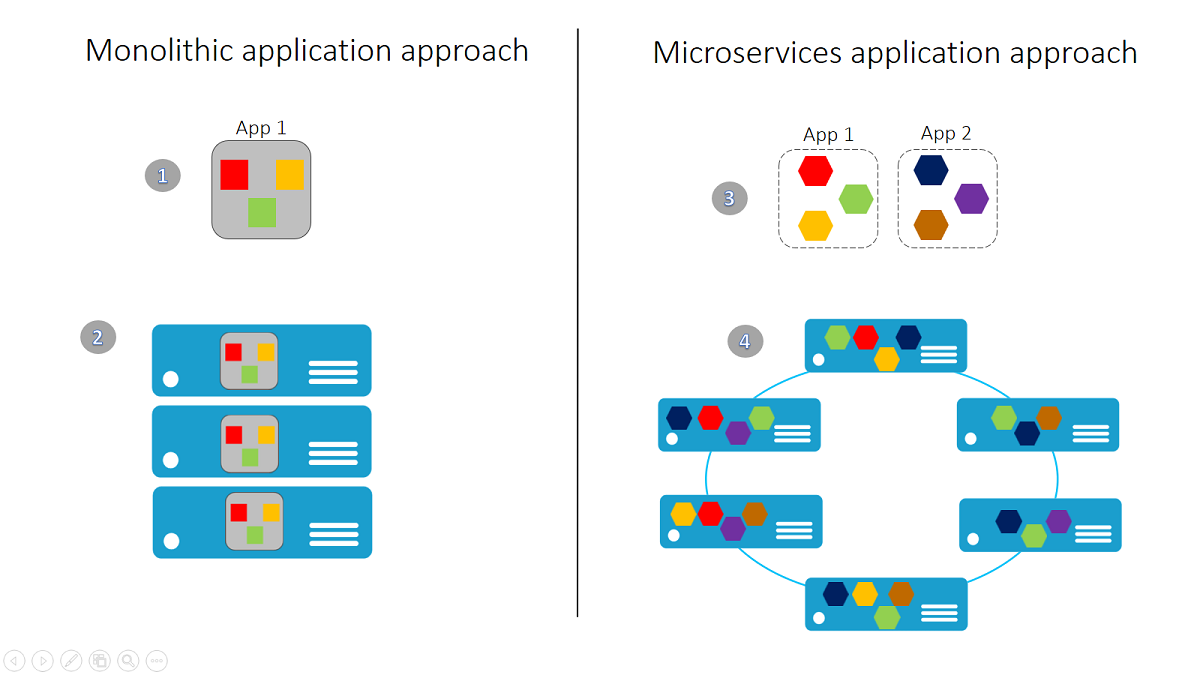
\includegraphics[width=0.9\textwidth]{monolithic_vs_micro}
	\caption{Sie sehen Unterschiede.\cite{irakli2016mic_arc}}
	\label{fig:trigo_funk}
\end{figure}

\begin{center}
	\begin{tabular}{|c|c|c|c|}
		Name & Vorname & Beruf & Wohnort \\
		\hline
		Erben & Thomas & Astronom & Bonn  \\
		Michael & Meier & & Stuttgart  \\
	\end{tabular}
\end{center}